In order to obtain the maximum and minimum value we need to solve the system of inequalities by adding slack variables. The equations now become:
\begin{align}
    x + 2y - Z =0
    \\
    x + 2y - S_1 = 100
    \\
    2x - y + S_2 = 0
    \\
    2x + y + S_3 = 200
\end{align}
The simplex table can be formed as
\begin{align}
    \myvec{x & y & s_1 & s_2 & s_3 & b \\\hline
    1 & $2$ & -1 & 0 & 0 & 50 \\
    2 & -1 & 0 & 1 & 0 & 0 \\
    2 & 1 & 0 & 0 & 1 & 200 \\\hline
    1 & 2 & 0 & 0 & 0 & 0}
\end{align}
The pivot element is 2 as the minimum ratio 50 occurs for y as the entering variable. Now reducing the simplex matrix we get
\begin{align}
    \myvec{x & y & s_1 & s_2 & s_3 & b \\\hline
    \frac{1}{2} & 1 & \frac{-1}{2} & 0 & 0 & 50 \\
    \frac{5}{2} & 0 & \frac{-1}{2} & 1 & 0 & 50 \\
    \frac{3}{2} & 0 & \frac{1}{2} & 0 & 1 & 150 \\\hline
    1 & 2 & 0 & 0 & 0 & 0}
\end{align}
This can be expressed in the form of matrix inequality for maximization and minimization respectively as:
\begin{align}
    \max_{\{x\}}\vec{c}^T\Vec{x}\\
    s.t \quad \Vec{A}\vec{x}\leq \vec{b} ; \Vec{x} \geq 0
    \\\min_{\{x\}}\vec{c}^T\Vec{x}\\
    s.t \quad \Vec{A}\vec{x}\geq \vec{b} ; \Vec{x} \geq 0
\end{align}
where
\begin{align}
    \Vec{c}=\myvec{1\\2}\\
    \Vec{A}=\myvec{1 & 2\\2 & -1\\2 & 1}\\
    \Vec{b}=\myvec{100\\0\\200}
\end{align}
Solving for Z by this reduction method we get
\begin{align}
    Max Z = 400 
    \\Min Z = 100
\end{align}
This can be solved in Python which generates the result as shown in Fig 1. 
\begin{figure}[h]
\renewcommand{\theenumi}{1}
\centering
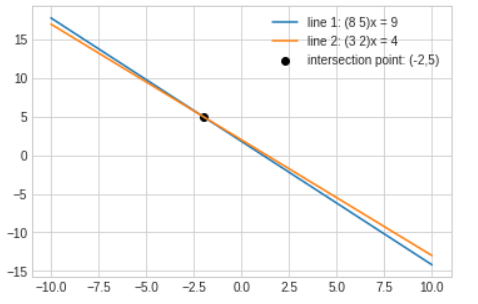
\includegraphics[width=\columnwidth]{./solutions/5/1/10/plot.png}
\caption{Plot from python code with Maxima and Minima points}
\label{eq:solutions/5/1/10/Fig:1}
\end{figure}
